\section{Lecture 5: Graph and Surface Codes - 17 February 2026}
Lecture Outline:
\begin{enumerate}[label=(\Roman*)]
    \item Graph States
    \item Graph Codes
    \item Surface Codes
\end{enumerate}

Last time: $S = \langle g_1, g_2, \cdots, g_{n-k} \rangle \rightarrow c(s)$ corrects $\{E_a\}$ if $\exists g \in S$ s.t. $Eg=-gE$, $\forall E = E_a^\dagger E_b$. If we have an element of the generator that anti-commutes with $E$, then we can detect it because it gives us a syndrome bit and that anti-commutation is the signature of an error having happened. 


\subsection{Graph States}
Goal: systematic construction of stabilizer codes\\
\textit{Codes have more than one state}
\begin{definition}
    A graph state (for graph $G$) is a stabilizer state with generator matrix in the symplectic representation
    \begin{equation}
        \left(\begin{array}{c|c} I & A \end{array}\right)
    \end{equation}
    Where $I$ (identity matrix) are the $X$ stabilizers and $A$ (adjacency) are the $Z$ stabilizers. $X$'s on vertices, and $Z$'s on edges.
\end{definition}
\begin{example}
    \begin{equation}
        \ket{\,%
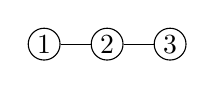
\begin{tikzpicture}[baseline=-0.6ex]
  \node[circle,draw,inner sep=1.2pt] (v1) at (0,0) {$1$};
  \node[circle,draw,inner sep=1.2pt] (v2) at (0.8,0) {$2$};
  \node[circle,draw,inner sep=1.2pt] (v3) at (1.6,0) {$3$};
  \draw (v1) -- (v2) -- (v3);
\end{tikzpicture}
\,} = \begin{pmatrix}
         X & Z & I \\
         Z & X & Z \\ 
         I & Z & X
     \end{pmatrix}
    \end{equation}
     Let $g_1 = XZI$, $g_2 = ZXZ$, $g_3=IZX$, this is a valid generator because there is an even amount of collisions of $X$'s and $Z$'s. 
\end{example}
\begin{example}
    \begin{equation}
        \Bigg|\,%
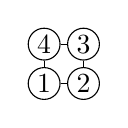
\begin{tikzpicture}[baseline=1.3ex, scale=0.5]
  % vertices
  \node[circle,draw,inner sep=1.2pt] (v1) at (0,0) {$1$};
  \node[circle,draw,inner sep=1.2pt] (v2) at (1,0) {$2$};
  \node[circle,draw,inner sep=1.2pt] (v3) at (1,1) {$3$};
  \node[circle,draw,inner sep=1.2pt] (v4) at (0,1) {$4$};
  % edges (a square)
  \draw (v1)--(v2)--(v3)--(v4)--(v1);
\end{tikzpicture}
\, \Bigg\rangle = \begin{pmatrix}
    X & Z& I& Z\\
     Z& X & Z& I\\
     I& Z & X & Z\\
     Z& I & Z & X
\end{pmatrix}
\end{equation}
\end{example}

\begin{fact}
    Graph states $\subset$ Stabilizer States. This can be seen because there are no minus signs. s
\end{fact}
There are multiple stabilizer states that correspond to the same graph. That homomorphism is a result of the following set of arguments which really shed light on the nature of stabilizer states themselves. 

\begin{definition}
    Local clifford (``LC") operators $\langle H, S \rangle$, where $H$ is Hadamard and $S$ is Phase $\sqrt{Z}$. 
\end{definition}
We take all possible strings of $H,S$ to strings which form a group, which is the single qubit Clifford group. (will come back to Clifford groups later). 
\begin{center}
    \begin{tabular}{c|c|c}
         $g$ & $HgH^\dagger$ & $SgS^\dagger$ \\
         \hline
         $X$ & $Z$ & $Y$ \\
         $Y$ & $-Y$ & $X$ \\
         $Z$ & $X$ & $Z$  
    \end{tabular}
\end{center}

\begin{claim}
    All stabilizer states are equivalent to a graph state under LC ops. (Check lecture notes after class on proofs). 
\end{claim}
Recall:
\begin{equation}
    S = \{g \in G \,|\, g\ket{\psi} = \ket{\psi} \}
\end{equation}
where $g$ is the stabilizer and $\ket{\psi}$ is the stabilizer state.
\begin{example}
    GHZ state = $\ket{000} + \ket{111}$, then $S = ZZI, IZZ, XXX$. What is $\ket{G}$?\\
    First we write down $S$ as a matrix. 
    \begin{equation}
        \begin{pmatrix}
            X &X &X \\
            I & Z& Z \\
            Z & Z& I 
        \end{pmatrix}
    \end{equation}
    We want $XXX$'s on the diagonal and $Z$'s on the outside. We'll use the local clifford operators. Labelling the columns $1,2,3$
    \begin{equation}
        \begin{pmatrix}
            X &X &X \\
            I & Z& Z \\
            Z & Z& I 
        \end{pmatrix}
        \xrightarrow{H_2H_3}
        \begin{pmatrix}
            X &Z & Z \\
            I & X& X \\
            Z & X& I 
        \end{pmatrix}
        \xrightarrow{c_2\leftrightarrow c_3}
        \begin{pmatrix}
            X &Z & Z \\
            I & X& X \\
            Z & I& X 
        \end{pmatrix}
        \xrightarrow{r_3\leftrightarrow r_2r_3} 
        \begin{pmatrix}
            X &Z & Z \\
            Z & X& I \\
            Z & I& X 
        \end{pmatrix}
    \end{equation}
    The graph state is then 
    \begin{equation}
        \Bigg| 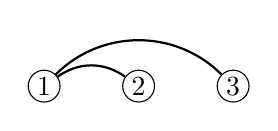
\begin{tikzpicture}[baseline=(n2.base)]
      \node[circle,draw,inner sep=1.2pt] (n1) at (0,0) {$1$};
      \node[circle,draw,inner sep=1.2pt] (n2) at (1.2,0) {$2$};
      \node[circle,draw,inner sep=1.2pt] (n3) at (2.4,0) {$3$};
    
      % same curves, but no arrowheads:
      \draw[line width=0.8pt] (n1) to[bend left=35] (n2);
      \draw[line width=0.8pt] (n1) to[bend left=45] (n3);
    \end{tikzpicture} \Bigg\rangle
    \end{equation}
    This is the same graph as the first one, so the first graph is a GHZ state. We're basically doing Gaussian elimination. 
\end{example}
\begin{example}
    Try yourself:
    \begin{equation}
        \begin{pmatrix}
            Z & Z & I \\
            I & Z & Z \\
            X & X & Y 
        \end{pmatrix}
    \xrightarrow{r_1r_3}
    \begin{pmatrix}
            X & X & Y \\
            Z & Z & I \\
            I & Z & Z 
        \end{pmatrix}
    \xrightarrow{H2S_3}
    \begin{pmatrix}
            X & Z & X \\
            Z & X & I \\
            I & X & Z 
        \end{pmatrix}
    \xrightarrow{H3}
    \begin{pmatrix}
        X & Z & Z \\
        Z & X & I \\
        I & X & X 
    \end{pmatrix}
    \xrightarrow{r_3 \rightarrow r_2r_3}
    \begin{pmatrix}
        X & Z & Z \\
        Z & X & I \\
        Z & Z & X 
    \end{pmatrix}
    \end{equation}
    
\end{example}
Remark: not all states are stabilizer states (ex $\ket{0 + \epsilon}$)\\ 
All states which can be $+1$ eigenstate of a Pauli operator. 
\begin{example}
    5-qubit code state $\ket{+_L}$ \\ 
    \begin{equation}
        \begin{pmatrix}
        X&Z&Z&X&I\\
        I&X&Z&Z&X\\
        X&I&X&Z&Z\\
        Z&X&I&X&Z\\
        X&X&X&X&Y
        \end{pmatrix}
    = \Bigg| 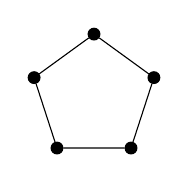
\begin{tikzpicture}[scale=0.4,
  every node/.style={circle, draw, fill=black, inner sep=1.5pt}
]

\node (n1) at (90:2)  {};
\node (n2) at (18:2)  {};
\node (n3) at (-54:2) {};
\node (n4) at (-126:2){};
\node (n5) at (162:2) {};

\draw (n1)--(n2)--(n3)--(n4)--(n5)--(n1);

\end{tikzpicture} \Bigg\rangle\end{equation} 
\end{example}

\begin{example}
    The graph for a 7 qubit code is a graph of half a cube, which is equivalent to 
    \begin{center}
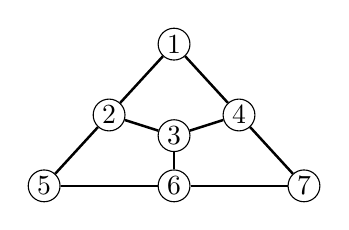
\begin{tikzpicture}[scale=0.75,
  every node/.style={circle, draw, fill=white, inner sep=1.2pt},
  e/.style={line width=0.9pt}
]

% --- triangle corners ---
\node (1) at (0,2.4) {1};
\node (5) at (-2.2,0) {5};
\node (7) at ( 2.2,0) {7};

% --- place 2,4,6 exactly on the triangle sides ---
% 2 on line segment 5--1, 4 on 1--7, 6 on 5--7
\node (2) at (-1.1,1.2) {2};
\node (4) at ( 1.1,1.2) {4};
\node (6) at (0,0) {6};

% interior node
\node (3) at (0,0.85) {3};

% --- outer triangle boundary as segmented sides ---
\draw[e] (5)--(2)--(1);
\draw[e] (1)--(4)--(7);
\draw[e] (5)--(6)--(7);

% --- interior edges (same as the original structure) ---
\draw[e] (2)--(3)--(4);
\draw[e] (3)--(6);

\end{tikzpicture}
\end{center}
\end{example}

Graph state construction circuits
\begin{enumerate}
    \item Each qubit starts in the $\ket{+}=H\ket{0} = $ vertices 
    \item Apply $CZ$-gate ($\Lambda_Z$) for every edge. 
\end{enumerate}
\begin{example}
    The circuit for the GHZ state: 
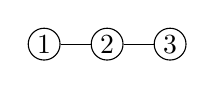
\begin{tikzpicture}[baseline=-0.6ex]
  \node[circle,draw,inner sep=1.2pt] (v1) at (0,0) {$1$};
  \node[circle,draw,inner sep=1.2pt] (v2) at (0.8,0) {$2$};
  \node[circle,draw,inner sep=1.2pt] (v3) at (1.6,0) {$3$};
  \draw (v1) -- (v2) -- (v3);
\end{tikzpicture}

\begin{center}
    \begin{quantikz}
        \lstick{$\ket{0}$} & \gate{H} \slice{$S_0$} & \ctrl{1}  \slice{$S_1$} & \qw \slice{$S_2$}& \qw  \\
        \lstick{$\ket{0}$} & \gate{H} & \ctrl{-1} & \ctrl{1} & \qw\\
        \lstick{$\ket{0}$} & \gate{H} & \qw & \ctrl{-1} & \qw
    \end{quantikz} \\
\end{center}
    Recall:
    \begin{quantikz}
        & \gate{X} & \ctrl{1} & \\
        &  &  \targ & \qw & \qw  
    \end{quantikz} = 
    \begin{quantikz}
        & \ctrl{1} & \gate{X} & \\
        &  \targ{} & \gate{X} &   
    \end{quantikz}
    and 
    \begin{quantikz}
        & \ctrl{1} & \\
        &  \targ{} &  
    \end{quantikz}
    = 
    \begin{quantikz}
        & \qw & \ctrl{1} &  & \\
         & \gate{H} &  \ctrl{-1} & \gate{H} &   
    \end{quantikz} \\
    Therefore, 
    \begin{quantikz}
        & \gate{X} & \ctrl{1} & \\
        &  & \ctrl{-1} & \qw 
    \end{quantikz} = 
    \begin{quantikz}
        & \ctrl{1} & \gate{X} & \\
        &  \ctrl{-1} & \gate{Z} &
    \end{quantikz}
 \\
At $S_0$, $S= \begin{pmatrix}
    X& I &I \\ I &X &I \\ I & I & X
\end{pmatrix}$, $\ket{\psi_0} = \ket{+}\ket{+}\ket{+}$ \\ 
At $S_1$, $S = \begin{pmatrix}
    X& X &I \\ I &Z &I \\ I & I & X
\end{pmatrix}$
At $S_2$, $S = \begin{pmatrix}
    X& Z &I \\ Z & X &I \\ I & I & X
\end{pmatrix}$
At $S_2$, $S = \begin{pmatrix}
    X& Z &I \\ Z & X & Z \\ I & Z & X
\end{pmatrix}$
\end{example}

\begin{theorem}
    $X\text{-}Z$ rule: 
    If you have a graph state and you apply a string of $X$'s to it, then the $X$ will be equivalent to something else in the same graph. 
    \begin{equation}
        X_k \ket{G} = \prod_{j \in neigh(k)} Z_j\ket{G}
    \end{equation}
    ($X$'s will cause a propagation of $Z$'s - just like the following circuit): 
     \begin{quantikz}
        & \gate{X} & \ctrl{1} & \\
        &  & \ctrl{-1} & \qw 
    \end{quantikz} = 
    \begin{quantikz}
        & \ctrl{1} & \gate{X} & \\
        &  \ctrl{-1} & \gate{Z} &
    \end{quantikz}
    The theorem states that bit flip errors can in turn into phase flip errors on a graph state.   
\end{theorem}
Suppose we had a error correction code that corrected possible phase flips, then it would equivalently correct bit flips, and vice-versa. 


\begin{example}
    $X$-$Z$ theorem: \\
    The graph 
    \begin{tikzpicture}[scale=1.2]
  % vertices (square)
  \node[circle,fill=black,inner sep=1.5pt] (v1) at (0,1) {};
  \node[circle,fill=black,inner sep=1.5pt] (v2) at (1,1) {};
  \node[circle,fill=black,inner sep=1.5pt] (v3) at (1,0) {};
  \node[circle,fill=black,inner sep=1.5pt] (v4) at (0,0) {};

  % edges
  \draw (v1)--(v2)--(v3)--(v4)--(v1);

  % label "x" near the top-left vertex
  \node[anchor=south east] at ($(v1)+(-0.1,0.05)$) {$X$};
\end{tikzpicture} 
    is equivalent to 
    \begin{tikzpicture}[scale=1.2]
  % vertices (square)
  \node[circle,fill=black,inner sep=1.5pt] (v1) at (0,1) {};
  \node[circle,fill=black,inner sep=1.5pt] (v2) at (1,1) {};
  \node[circle,fill=black,inner sep=1.5pt] (v3) at (1,0) {};
  \node[circle,fill=black,inner sep=1.5pt] (v4) at (0,0) {};

  % edges
  \draw (v1)--(v2)--(v3)--(v4)--(v1);

  % label "Z" near the top-left vertex
  \node[anchor=south west] at ($(v2)+(-0.1,0.05)$) {$Z$};
  \node[anchor=north east] at ($(v4)+(-0.1,0.05)$) {$Z$};
\end{tikzpicture} 
\end{example}

This $X$-$Z$ rule led to Codeword Stabilized codes (CWS) codes. This is the to this day the largest systematic construction of non-stabilizing codes.



\subsection{Graph Codes}
(will be going quick because this is not so useful - but conceptually important) \\ 
Goal: Represent subspaces not just states \\
There is a degeneracy in graph representation, because if we flip the sign of any of these generators $g_k \rightarrow -g_k$, we get the same graph. Changing the sign of the generators changes the eigenvalue, like we go from 0 to 1 in a state.  \\
Recall: if $\ket{\psi}$ is a stabilizer state, 
\begin{equation}
    U \ket{\psi} = Ug \ket{\psi} = Ug U^\dagger U \ket{\psi} 
\end{equation}
then $UgU^\dagger$ are stabilizer transforms.

\begin{definition}
    Graph basis for $\ket{G}$ is \begin{equation}
        \{\ket{G_s}= Z^S \ket{G} \,|\, S = \{0,1\}^n \}
    \end{equation} 
    $Z^S$ causes sign change. so for $\ket{G} = \langle g_1, g_2, \ldots, g_n\rangle$, $\ket{G_s} = \langle (-1)^{S_1}g_1, (-1)^{S_2}g_2, \ldots, (-1)^{S_n}g_n\rangle$
\end{definition}

\begin{definition}
    A \textbf{graph code} $C(G,\{S_1,S_2, \ldots\}$ is the space spanned by $\{\ket{GS_1}, \ket{GS_2}, \ldots\}$. 
\end{definition}

\begin{fact}
    Graph codes $\subset$ Stabilizer codes
\end{fact}

\begin{example}
    \begin{equation}
        S = \begin{pmatrix}
            X&I&I \\ I&X&I \\ I&I&X
        \end{pmatrix}
    \end{equation}
    which corresponds to a graph of 3 vertices (no edges)
    $\ket{G} = \ket{+++}$, $Z^{\otimes 3} \ket{G} = \ket{---}$
\end{example}

\begin{example}
    \begin{equation}
        \Bigg| 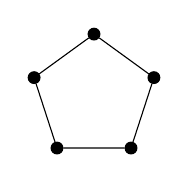
\begin{tikzpicture}[scale=0.4,
  every node/.style={circle, draw, fill=black, inner sep=1.5pt}
]

\node (n1) at (90:2)  {};
\node (n2) at (18:2)  {};
\node (n3) at (-54:2) {};
\node (n4) at (-126:2){};
\node (n5) at (162:2) {};

\draw (n1)--(n2)--(n3)--(n4)--(n5)--(n1);

\end{tikzpicture} \Bigg\rangle = \ket{G}
    \end{equation} and $Z^{\otimes 5} \ket{G} \Rightarrow [[5,1,3]]$ code \\ We only have one qubit.
\end{example}
This gives us a systematic way of getting arbitrary codes. 

\begin{example}
    Shor code graph: \\
    \begin{center}
    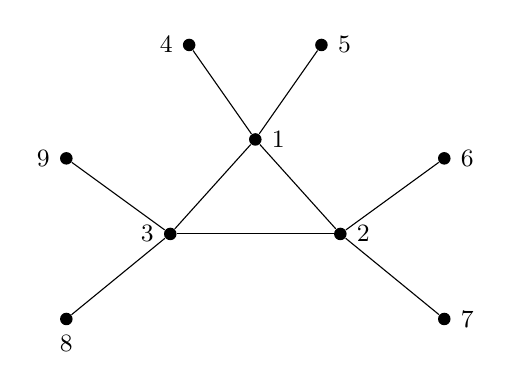
\begin{tikzpicture}[scale=1.2, every node/.style={font=\small}]
  % --- Nodes (positions chosen to match the drawing) ---
  \node[circle, fill=black, inner sep=1.6pt, label=right:$1$] (v1) at (0,1.2) {};
  \node[circle, fill=black, inner sep=1.6pt, label=left:$4$]  (v4) at (-0.7,2.2) {};
  \node[circle, fill=black, inner sep=1.6pt, label=right:$5$] (v5) at (0.7,2.2) {};

  \node[circle, fill=black, inner sep=1.6pt, label=left :$3$] (v3) at (-0.9,0.2) {};
  \node[circle, fill=black, inner sep=1.6pt, label=right:$2$]      (v2) at (0.9,0.2) {};

  \node[circle, fill=black, inner sep=1.6pt, label=left:$9$] (v9) at (-2.0,1.0) {};
  \node[circle, fill=black, inner sep=1.6pt, label=below:$8$] (v8) at (-2.0,-0.7) {};

  \node[circle, fill=black, inner sep=1.6pt, label=right:$6$] (v6) at (2.0,1.0) {};
  \node[circle, fill=black, inner sep=1.6pt, label=right:$7$] (v7) at (2.0,-0.7) {};

  % --- Edges (matching the picture) ---
  \draw (v1)--(v4);
  \draw (v1)--(v5);

  \draw (v1)--(v3);
  \draw (v1)--(v2);

  \draw (v3)--(v2);   % horizontal base edge

  \draw (v3)--(v9);
  \draw (v3)--(v8);

  \draw (v2)--(v6);
  \draw (v2)--(v7);
\end{tikzpicture}
\end{center}
    \hspace*{1.5cm} $=Z_1Z_2Z_3 \ket{G} \Rightarrow [[9,1,3]]$ Shor code.  
\end{example}


\subsection{Surface Codes}
Goal: Define a stabilizer code s.t. if qubits are on a surface, all generators of the code are local operations. \\
Concept: \\
\begin{center}
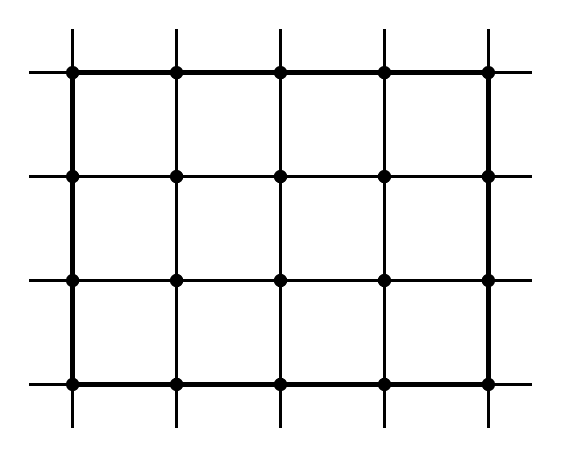
\begin{tikzpicture}[scale=1.1]
  % --- grid size (number of cells) ---
  \def\Nx{4}    % columns of cells
  \def\Ny{3}    % rows of cells
  \def\s{1.2}   % spacing
  \def\ext{0.5}% overshoot amount (in same units as coords)

  % --- draw vertical lines with overshoot ---
  \foreach \i in {0,...,\Nx} {
    \draw[line width=1.2pt]
      (\i*\s,-\ext) -- (\i*\s,\Ny*\s+\ext);
  }

  % --- draw horizontal lines with overshoot ---
  \foreach \j in {0,...,\Ny} {
    \draw[line width=1.2pt]
      (-\ext,\j*\s) -- (\Nx*\s+\ext,\j*\s);
  }

  % --- outer boundary (frame) ---
  \draw[line width=1.8pt] (0,0) rectangle (\Nx*\s,\Ny*\s);

  % --- dots at each intersection (inside the frame) ---
  \foreach \i in {0,...,\Nx} {
    \foreach \j in {0,...,\Ny} {
      \fill (\i*\s,\j*\s) circle (2.2pt);
    }
  }
\end{tikzpicture}
\end{center}

Edges $E$, Vertices $V$, Faces/Plaquette $F/P$;
The qubits be on edges. \\
Periodic boundary conditions = toric code \\
Planar = surface code \\
The goal of all of these constructions is to find a way to represent a stabilizer state, meaning we can write down a series of stabilizer generators which all commute with each other. (This is the fun game with simple rules - just find a systematic way of getting a bunch of stuff commuting and we get a code.) \\

The state generator which will be the products around the edges corresponds to the vertex $v$
\begin{equation}
    A_v = \prod_{e \sim v} X_e \text{ and } B_p =  \prod_{e \sim f} Z_e
\end{equation}

\begin{center}
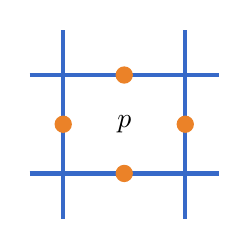
\begin{tikzpicture}[scale=0.5]
  % colors close to the figure
  \definecolor{lineblue}{RGB}{55,105,200}
  \definecolor{dotorange}{RGB}{235,130,40}

  % parameters
  \def\L{2.4}     % half-length of each long line segment
  \def\xs{1.55}   % x-position of the two vertical grid lines
  \def\ys{1.25}   % y-position of the two horizontal grid lines
  \def\r{0.22}    % dot radius

  % grid lines (2 vertical + 2 horizontal)
  \draw[line width=1.5pt, lineblue] (-\xs,-\L) -- (-\xs,\L);
  \draw[line width=1.5pt, lineblue] ( \xs,-\L) -- ( \xs,\L);
  \draw[line width=1.5pt, lineblue] (-\L,-\ys) -- (\L,-\ys);
  \draw[line width=1.5pt, lineblue] (-\L, \ys) -- (\L, \ys);

  % dots (midpoints of each side of the central square)
  \fill[dotorange, line width=1.5pt] (0, \ys)  circle (\r);   % top
  \fill[dotorange, line width=1.5pt] (0,-\ys)  circle (\r);   % bottom
  \fill[dotorange,  line width=1.5pt] (-\xs,0)  circle (\r);   % left
  \fill[dotorange, line width=1.5pt] ( \xs,0)  circle (\r);   % right

  % label
  \node at (0,0) {$p$};
\end{tikzpicture}
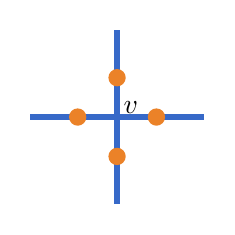
\begin{tikzpicture}[scale=0.5]
  % colors
  \definecolor{lineblue}{RGB}{55,105,200}
  \definecolor{dotorange}{RGB}{235,130,40}

  % parameters
  \def\L{2.2}   % half-length of the cross arms
  \def\r{0.22}  % radius of the dots

  % cross
  \draw[line width=2pt, lineblue] (-\L,0) -- (\L,0);
  \draw[line width=2pt, lineblue] (0,-\L) -- (0,\L);

  % dots (top, bottom, left, right)
  \fill[dotorange,  line width=1.5pt] (0, 1.0) circle (\r);
  \fill[dotorange, line width=1.5pt] (0,-1.0) circle (\r);
  \fill[dotorange, line width=1.5pt] (-1.0,0) circle (\r);
  \fill[dotorange, line width=1.5pt] ( 1.0,0) circle (\r);

  % label
  \node at (0.35,0.25) {$v$};
\end{tikzpicture}
\end{center}


\begin{claim}
    All $B_p, A_v$ commute if they share no qubits, i.e. disjoint. If there's an overlap, they share 2 edges, therefore $B_p, A_v$ commute. We always either share 0 or 2 edges. They commute because the two Pauli operators all multiply out together to give identity. 
\end{claim}

How many qubits are encoded? Let's look at how many degrees of freedom left over. We know that $k = n - |g|$ where $g$ is the number of independent generators. If we take two faces and we take their product: 1) if they're on top of each other, we get the same to each other; 2) if they're adjacent to each other, we get a bigger face; suppose we take all the faces and multiply them together i.e.
\begin{equation}
    \prod_p B_p = \mathbb{1}
\end{equation}
Similarly,
\begin{equation}
    \prod_v A_v = \mathbb{1}
\end{equation}
We have overcounted the number of independent generators. Given an $L \times L$ lattice, 
then 
\begin{align}
    &\text{number of faces } = L^2 \\
    &\text{number of vertices } = L^2 \\
    &\text{number of edges = qubits} = 2L^2
\end{align}
Therefore, 
\begin{equation}
    k = 2L^2 - [L^2 - 1 + L^2 -1] = 2
\end{equation}
where the $-1$ comes from overcounting by 1 since the product is identity. \\
\textit{For the torus code, it is easy to see we have 2 qubits because we have two non-contractible loops that go around the major and minor axis.} \\

Geometry of how these loops work: \\

Imagine if we have two faces next to each other, and we have face $f_1$ and $f_2$. $f_1$ has a $Z$ on the shared qubit and $f_2$ has a $Z$ on the shared qubit. $ZZ = I$, therefore we have 1 larger face.  \\ 

\begin{center}
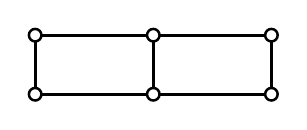
\begin{tikzpicture}[scale=0.75]
  % styles
  \tikzset{
    v/.style={circle, fill=white, draw=black, line width=0.9pt, inner sep=1.6pt},
    e/.style={draw=black, line width=1.2pt}
  }

  % coordinates (two squares sharing the middle vertical edge)
  \coordinate (A) at (0,1);    % top-left
  \coordinate (B) at (2,1);    % top-middle
  \coordinate (C) at (4,1);    % top-right
  \coordinate (D) at (0,0);    % bottom-left
  \coordinate (E) at (2,0);    % bottom-middle
  \coordinate (F) at (4,0);    % bottom-right

  % edges
  \draw[e] (A)--(B)--(C);
  \draw[e] (D)--(E)--(F);
  \draw[e] (A)--(D);
  \draw[e] (B)--(E);
  \draw[e] (C)--(F);
  \draw[e] (D)--(A); % (optional, same as A--D; remove if you want no double-draw)
  \draw[e] (A)--(B)--(E)--(D)--cycle; % left square
  \draw[e] (B)--(C)--(F)--(E)--cycle; % right square

  % vertices
  \node[v] at (A) {};
  \node[v] at (B) {};
  \node[v] at (C) {};
  \node[v] at (D) {};
  \node[v] at (E) {};
  \node[v] at (F) {};
\end{tikzpicture}, $f_1f_2 = $
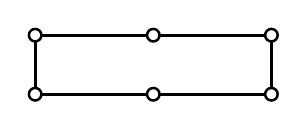
\begin{tikzpicture}[scale=0.75]
  \tikzset{
    v/.style={circle, fill=white, draw=black, line width=0.9pt, inner sep=1.6pt},
    e/.style={draw=black, line width=1.2pt}
  }

  % coordinates (outer rectangle corners + the two middle vertices)
  \coordinate (A) at (0,1);    % top-left
  \coordinate (B) at (2,1);    % top-middle (vertex only)
  \coordinate (C) at (4,1);    % top-right
  \coordinate (D) at (0,0);    % bottom-left
  \coordinate (E) at (2,0);    % bottom-middle (vertex only)
  \coordinate (F) at (4,0);    % bottom-right

  % outer rectangle edges ONLY (no middle vertical line)
  \draw[e] (A)--(C)--(F)--(D)--cycle;

  % vertices (keep all 6)
  \node[v] at (A) {};
  \node[v] at (B) {};
  \node[v] at (C) {};
  \node[v] at (D) {};
  \node[v] at (E) {};
  \node[v] at (F) {};
\end{tikzpicture}
\end{center}

\begin{equation}
    \prod_f B_f^\beta = \text{closed loops of } Z\text{'s } 
\end{equation}


For vertices, if we go through some loop path $\beta$
\begin{center}
\begin{tikzpicture}[scale=1.1]
  % styles
  \tikzset{
    wire/.style={line width=1.2pt},
    boundary/.style={line width=1.0pt, dashed, dash pattern=on 3pt off 2pt},
    dot/.style={circle, draw, fill=white, inner sep=1.6pt, line width=1pt},
  }

  % junction centers
  \coordinate (A) at (0,1);    % left junction
  \coordinate (B) at (3,1);    % upper-right junction (circled)
  \coordinate (C) at (3,-1);   % lower-right junction

  % main connecting "wires"
  \draw[wire] (A) -- (B);
  \draw[wire] (B) -- (C);

  % draw plus-junctions (little crosses)
  % at A
  \draw[wire] ($(A)+(-1.55,0)$) -- ($(A)+(0.55,0)$);
  \draw[wire] ($(A)+(0,-1.55)$) -- ($(A)+(0,1.)$);

  % at B (plus + circle)
  \draw[wire] ($(B)+(-0.75,0)$) -- ($(B)+(1.25,0)$);
  \draw[wire] ($(B)+(0,-0.75)$) -- ($(B)+(0,1.00)$);

  % at C
  \draw[wire] ($(C)+(-1.20,0)$) -- ($(C)+(1.25,0)$);
  \draw[wire] ($(C)+(0,-1.25)$) -- ($(C)+(0,0.75)$);

  % dashed "L-shaped" boundary with an inner corner
  \draw[boundary, rounded corners=8pt]
    (-0.9, 1.55) -- (3.75, 1.55) -- (3.75,-1.55) -- (2.35,-1.55)
    -- (2.35, 0.25) -- (-0.9,0.25) -- cycle;
\end{tikzpicture}
\end{center}

\begin{equation}
    \prod_v A_v^\beta = \text{closed loops of } X\text{'s in the dual lattice}
\end{equation}

We can contract any loops, except for loops that are topologically non-trivial (like they wind all the way around). How much effort does it take to contract a loop? First, 
\begin{equation}
\text{the number of qubits = number of non-contractable loops}    
\end{equation}
We now have a well defined notion of distance:
\begin{equation}
\text{Distance = length of non-contractable loops}  
\end{equation}
If you imagine that the error is that each one of these edges gets an $X$ or a $Z$ error with some probability $p$, the only time you have an error that would go bad is if you went too far across, and you can't tell if it was actually going all the way around or not, because it becomes misidentified as a non-contractible loop. \\
The loop distance $L\sim \sqrt{n}$, since $n$ goes as $L^2$. So $L$ being the length across the lattice tells you about the number of errors before you start going bad. \\

Scaling properties of when the error correction code would fail: \\
Let $P_{fail}$ be the failure probability rate of decoding (syndrome) and recovery ($R$). 
\begin{equation}
    P_{fail} = C \left(\frac{P}{P_{th}}\right)^{\frac{d+1}{2}}
\end{equation}
where $C$ is a constant that depends on the hardware and decoding error, $P$ is the physical error rate (logical qubit), $P_{th}$ is the property of the code, i.e., the break-even point (threshold probability - will come back to fault-tolerant quantum computing). We can think $P_{th}$ as the number of fault paths in the code decoder. \\
In summary, $P_{th}$ scales with size of code, $P$ has to do with the number of qubits. \\

$d = \#$ physical errors to make non-contractable loop, code can correct up to $t = \frac{d-1}{2}$ errors.  

Matching algorithm: take the syndrome that you get and turn it into the error that you think happened. Perfect matching is an exhaustive way to do that. 